\documentclass[../main.tex]{subfiles}
\begin{document}
\section{Results}
\label{sec:results}

...

Sample of ~200,000 households of ethnically Danish origin (all household members are of Danish ethnicity) from 2017-2019 who earn from DKK 100,000 to 1,500,000 DKK. They \textit{all} at some point experience getting a new non-west neighbor (defined as a household with at least one member from non-west origin). Apart from neighborhood-by-quarter FE, no further controls are added. Given that people are in a state of flow, I have devised a "stable" definition of a household.

Borrowing from the graph theory literature, I first identify connected components, or individuals, who overlap in space and time. However, this only gives me transitive connections (example), so I have devised an algorithm (?) that uses \textbf{familie\_id} from the \textbf{BEF} table to define the "best" partition. This is done via calculating temporal and social (whether you are partners or parents/children) edge weights and subsequently maximize these. To illustrate, consider the figure below that illustrates this approach. A connected component definition of a household would define the whole graph as a single household. Maximizing edge weights would yield three different "stable" households instead of one.


\begin{figure}[H]
    \centering
    \caption{Household definition}
    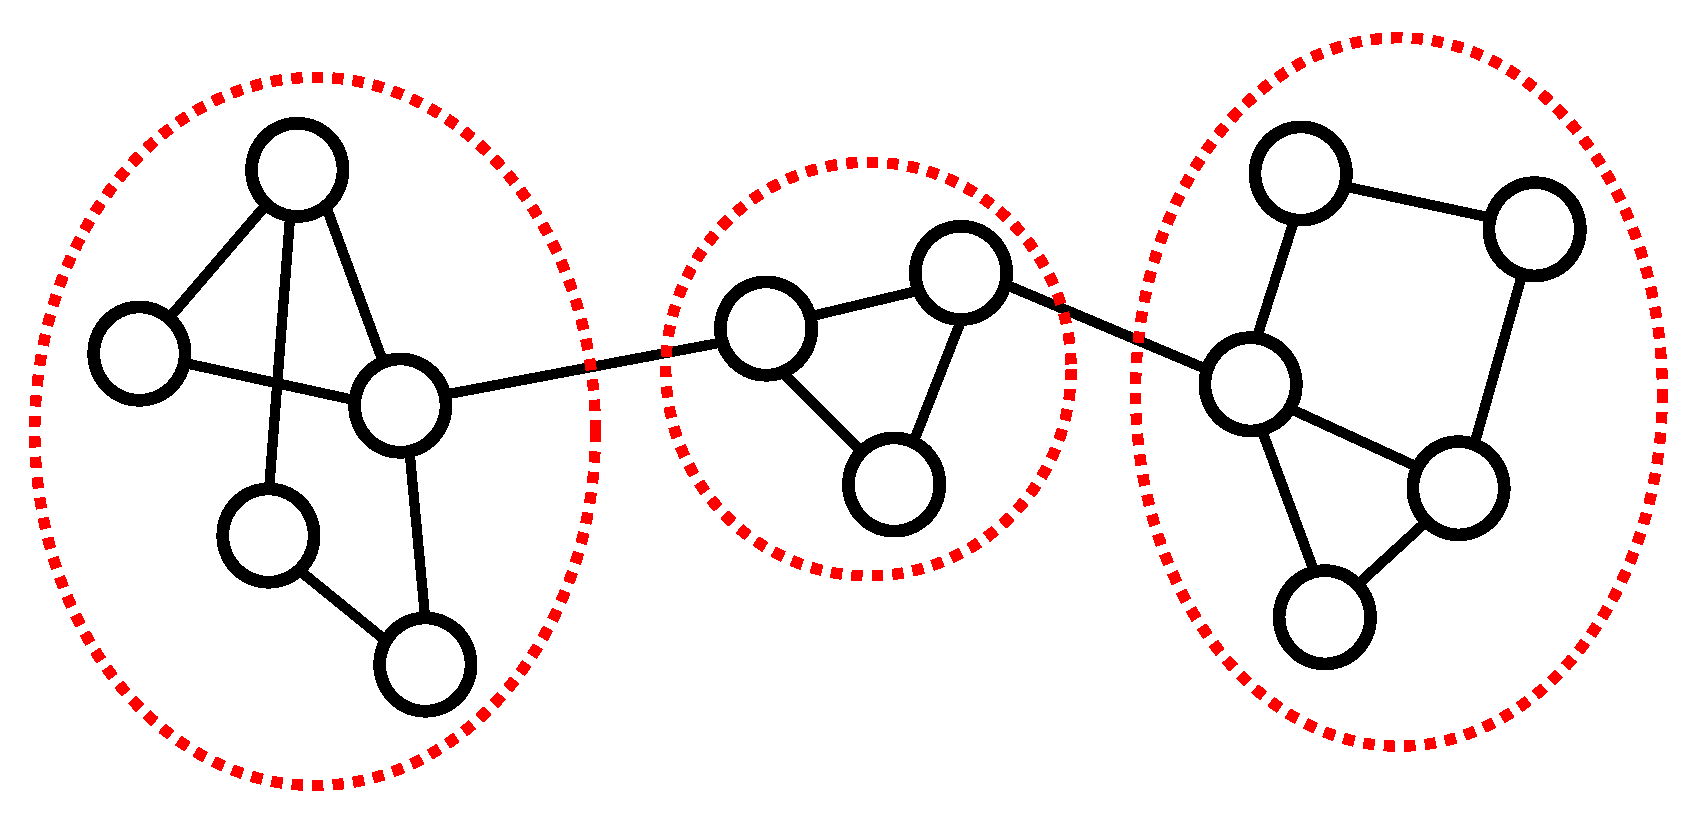
\includegraphics[width=0.4\linewidth]{figs/temporal_community_detection.png}
\end{figure}

\begin{table}[H]
    \caption{Regression output}
    \centering
    \resizebox{0.8\textwidth}{!}{\centering
\begin{tabular}[t]{lc}
\toprule
  & Moved within 2 years (=100)\\
\midrule
I\_nearest & \num{0.318}*\\
 & (\num{0.084})\\
I\_near & \num{0.210}**\\
 & (\num{0.035})\\
I\_far\_20 & \num{0.203}\\
 & (\num{0.098})\\
I\_far\_30 & \num{0.045}\\
 & (\num{0.043})\\
\midrule
I_{nearest} - I_{near} = 0 & 0.1079\\
 & (0.1006)\\
\midrule
Num.Obs. & \num{813713}\\
Mean of Dependent Variable & 12.76\\
Neighborhood-by-quarter FE & X\\
\bottomrule
\multicolumn{2}{l}{\rule{0pt}{1em}Significance levels: *** p $<$ 0.01, ** p $<$ 0.05 * p $<$ 0.1}\\
\multicolumn{2}{l}{\rule{0pt}{1em}Standard errors in parenthesis. Standard errors are clustered at the municipality-year level.}\\
\multicolumn{2}{l}{\rule{0pt}{1em}Neighborhoods are heuristically aggregated from Nabolagsatlas.dk to contain a minimum of 500 people.}\\
\end{tabular}}
    \label{tab:my_label}
\end{table}

\end{document}